% Section 1 : Contexte du stage
	\section{Contexte du stage}
	\subsection{L'entreprise}
	\subsubsection{Inria}
		L'Inria (Institut national de recherche en informatique et en automatique) est un institut de recherche crée en 1967 dans le cadre du plan Calcul. Il compte 2400 collaborateurs et 1200 doctorants travaillant dans les 8 centres de recherche répartis dans toute la France, et jouit d'un fort rayonnement à l'international. J'ai effectué mon stage dans le centre Inria de Lille, au sein de l'équipe RMoD.
	\subsubsection{RMoD}
	RMoD est une équipe de recherche en \textbf{génie logiciel} basée dans le centre Inria de Lille - Nord Europe et dirigée par Stéphane Ducasse. Son principal but est l'évolution des systèmes sur le long terme, effectuée sur 2 axes : l'évolution de systèmes existants (appelés également systèmes legacy) , et la création de nouveaux systèmes aisément améliorables.
	
	\subsection{Technologies employées}
	\subsubsection{Pharo}
	Pharo est un langage de programmation open source créé en 2008 par l'équipe RMoD, issu d'un fork de Squeak. Il est basé sur une machine virtuelle (VM) écrite en grande partie en Pharo lui-même, ce qui lui donne la capacité d'être multiplateforme (Mac OS X, Windows, Linux, iOS, Android). Sa politique impose que ses contributeurs publient leur code sous licence MIT.
	
	\paragraph{Fonctionnalités :}
	Basé sur Smalltalk, Pharo en possède les principales caractéristiques:
	\begin{itemize}
		\item Le système est réflexif.
		\item Le typage est dynamique.
		\item Pharo est implémenté suivant le paradygme objet
		\item L'héritage est simple.
		\item La gestion de la mémoire se fait automatiquement au moyen d'un garbage collector (GC)
	\end{itemize}

	\paragraph{Syntaxe :}
	La figure suivante représente la syntaxe complète de Pharo :
	
	\begin{figure}
		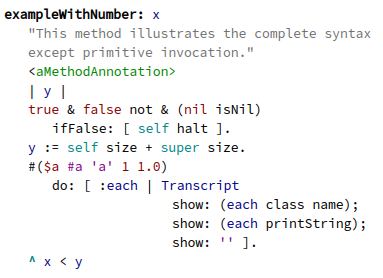
\includegraphics[width=12cm]{./img/pharo_syntax.png}
		\caption[pharosyntax]{La syntaxe complète de Pharo}
	\end{figure}

	\paragraph{Live Programming :}
	L'un des principaux intérêts de Pharo est qu'il n'est pas nécessaire de recompiler tout le code en cas de modification. Il est par exemple possible de coder au sein du debugger : On écrit un test, on le lance, une erreur apparait (le message envoyé n'existe pas), on peut alors ouvrir le debugger, implémenter la méthode correspondante, compiler à la volée et reprendre le cours de l'exécution comme si rien ne s'était produit.
	
	\paragraph{}
	Pharo est actuellement disponible dans sa version 6.0, sortie le 6 juin 2017.

	\subsubsection{git}
	Git est un logiciel libre de gestion de versions décentralisé créé par Linus Torvalds, et distribué sous la licence publique générale GNU (GPL-2.0). Il est particulièrement utile pour gérer les modifications apportées à un projet grâce à un système de commits et de branches, surtout si il est couplé à un service en ligne capable de le gérer (par exemple github, pour ne citer que le plus connu).
